\chapter{Iterated Products of Orthogonal Projections in Hilbert Space}\label{chapt:Iterated_Products_of_Projections_in_Hilbert_Space}In this chapter, we focus on the convergence of the iterated products of orthogonal projections in Hilbert Space. This classical result was first estabilished for two orthogonal projections by \emph{J.Von Neumann}\cite{JN33} in 1933 in the form of the following theorem:
\begin{theorem}
Let $X$ be a Hilbert Space, and $M_1,M_2$ be closed subspaces of $X$. If $P_{M_i}$ is an orthogonal proection on $M_i$ for eacu $i=1,2$, and $P_{M}$ is the orthogonal projection on the closed subspace $M=M_1\cap M_2$, then for each $x\in X$,
$$\lim_{n\rightarrow\infty}(P_{M_1}P_{M_2})^n(x)=P_{M}(x).$$
\end{theorem}

We can simply demonstrate this beautiful result in the two-dimensional case:

Let $M_1$ and $M_2$ be the two straight lines as shown in the diagram below, and $x$ be an arbitrary element from $\mathbb{R}^2$. If we define an alternating sequences $\{x_n\}$ by
$$x_0=x,$$
$$x_{2n+1}=P_{M_1}(x_{2n}),$$
$$x_{2n}=P_{M_2}(x_{2n-1})=(P_{M_1}P_{M_2})^n(x_0)), $$
then $\lim_{n\rightarrow\infty}x_n=P_{M}(x).$
\begin{figure}[h]
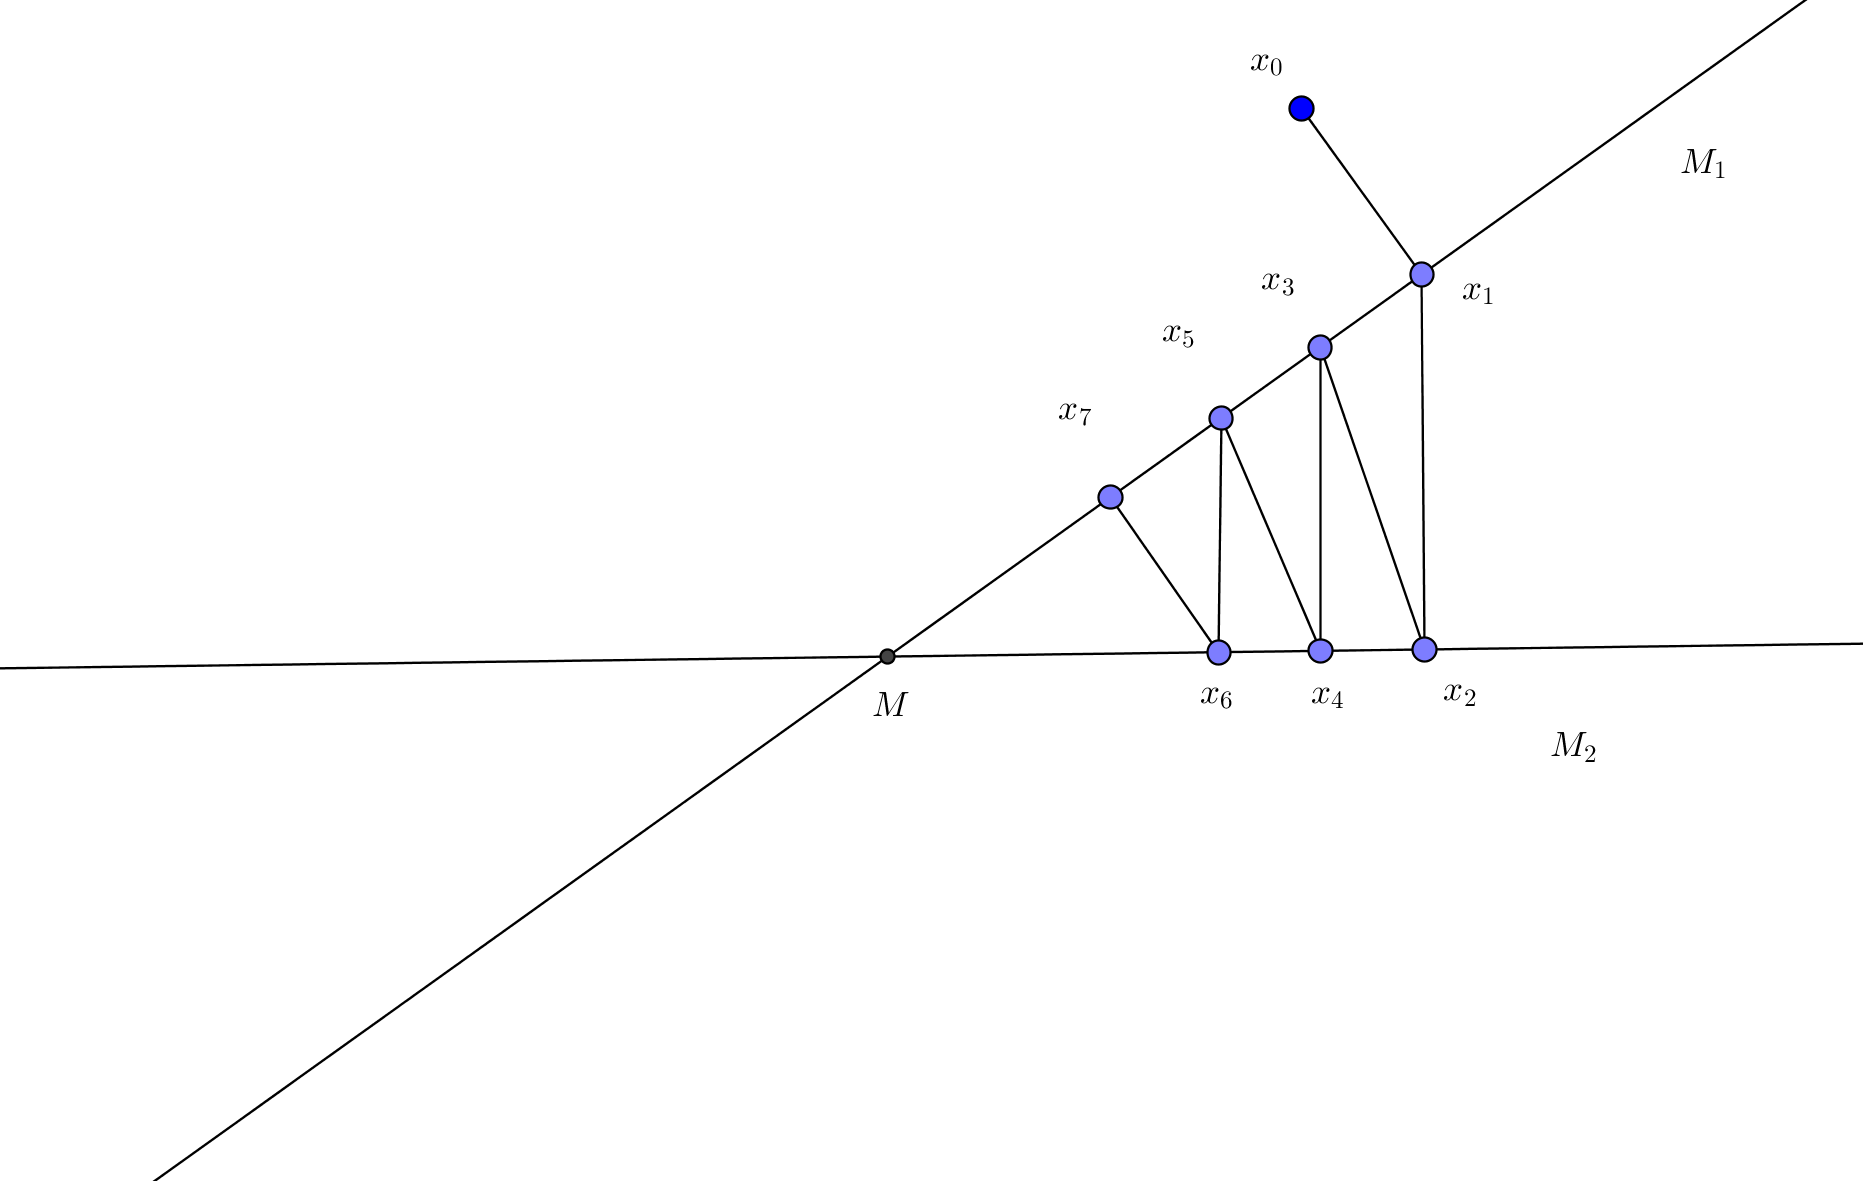
\includegraphics[width=140mm,scale=0.8]
{2d_demo.png}
\end{figure}
\par
 The same theorem was also found by \emph{Nakano} \cite{NN53} in 1953 and \emph{Wiener}\cite{NW55} in 1955. Indeed, the result is also true for any arbitrary finite number of orthogonal projections as shown in \emph{Halperin's} work \cite{IH62} in 1962.
